\documentclass{article}
\usepackage{parskip}
\usepackage{amsmath}
\usepackage[dvipdfmx]{graphicx}
\usepackage{cleveref}
\begin{document}

ある長方形を3つの長方形に分割する方法は,
ある1辺に平行な2本の線分によって分割する方法(\cref{type-i})か,
各辺にそれぞれ平行な1本ずつの線分によって分割する方法(\cref{type-t})のいずれかのみである。
これらをそれぞれI型,T型と呼ぶことにする。

\begin{figure}[h]
    \begin{center}
        \begin{tabular}{c}
            \begin{minipage}{0.33\hsize}
                \begin{center}
                    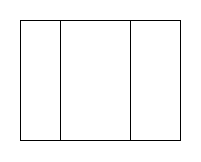
\includegraphics[width=100pt]{type-i.png}
                    \caption{I型}
                    \label{type-i}
                \end{center}
            \end{minipage}

            \begin{minipage}{0.33\hsize}
                \begin{center}
                    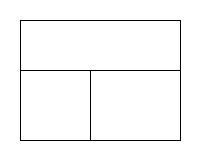
\includegraphics[width=100pt]{type-t.png}
                    \caption{T型}
                    \label{type-t}
                \end{center}
            \end{minipage}
        \end{tabular}
    \end{center}
\end{figure}


\end{document}
